% Exemple de CV utilisant la classe moderncv
% Style classic en bleu
% Article complet : http://blog.madrzejewski.com/creer-cv-elegant-latex-moderncv/

\documentclass[11pt,a4paper]{moderncv}




\moderncvtheme[blue]{classic}                
\usepackage[utf8]{inputenc}
\usepackage[top=0.5cm, bottom=0.5cm, left=1.5cm, right=1.5cm]{geometry}
%anciennement:\usepackage[top=1.1cm, bottom=1.1cm, left=2cm, right=2cm]{geometry}

\usepackage{graphicx}
\usepackage{float}
\usepackage{graphicx}


% Largeur de la colonne pour les dates
\setlength{\hintscolumnwidth}{2.5cm}
\definecolor{color1}{rgb}{0.22,0.45,0.70}% light blue
\definecolor{color2bis}{rgb}{0.33, 0.33, 0.33}% grey


\firstname{Thomas}
\familyname{Lentali}
\title{Data Scientist\\Recherche Opérationnelle}              
\email{thomas.lentali@gmail.com}                      
\phone{\textbf{06 16 24 58 68}} 
\extrainfo{05/12/1988 (27 ans) -- Permis B}
\address{8 avenue Bon Air - D105}{33700 Mérignac}
\photo[58pt][0pt]{QRcodeA.png}

\begin{document}
\maketitle

\section{Expériences professionnelles / stages}

\cventry{\textcolor{color2bis}{2016\\Mars-Sept.\\(6 mois)}}{Stage fin de Master}{Cdiscount}{Bordeaux}{France}{Machine learning et analyse statistique dans le service responsable de la pertinence du moteur de recherche du site Cdiscount.\\ 
\textit{\underline{Ciblage marketing}:} analyse comportementale et amélioration
de la pertinence moteur (test AB), personnalisation client de la page d'acceuil (classification)\\
\textit{\underline{Valorisation de données géographique}:} prédiction des achats
par zone géographique (machine learning), analyse statistique: croisement
données INSEE/Cdiscount, création d'un outil de géocoding (géomatique)\\
\textit{\underline{Projet concours Innovation Interne}:} proposition d'un plan
opérationnel de mise en place d'un nouveau service aux clients: système d'anticipation de stockage de produits en points relais pour développer la livraison express.\\
\underline{Savoir-Être} : Esprit d'équipe, organisation (agile), rigueur.
\newline{}}

\cventry{\textcolor{color2bis}{2016\\Janvier-Mars\\(3 mois)}}{Projet
  professionnel}{Abracadacook}{Bordeaux}{France}{Développement d'outils de
  détection d'information dans un texte (détection d'anomalie) et
  classification.\\
\underline{Savoir-Être} : écoute, autonomie, capacité d'adaptation.
\newline{}}


\cventry{\textcolor{color2bis}{2015\\Juin-Août\\(2 mois)}}{Stage
  volontaire}{Cartegie}{Bordeaux}{France}{Sourcing et mise en place d'outils de machine learning (classification supervisée) au sein d'un parc de données sous Spark.\\
\underline{Savoir-Être} : Polyvalence, problem solving, proactivité.
\newline{}}

\section{Compétences}
% \vspace{0.1mm}
\begin{minipage}{\textwidth}
  \centering
  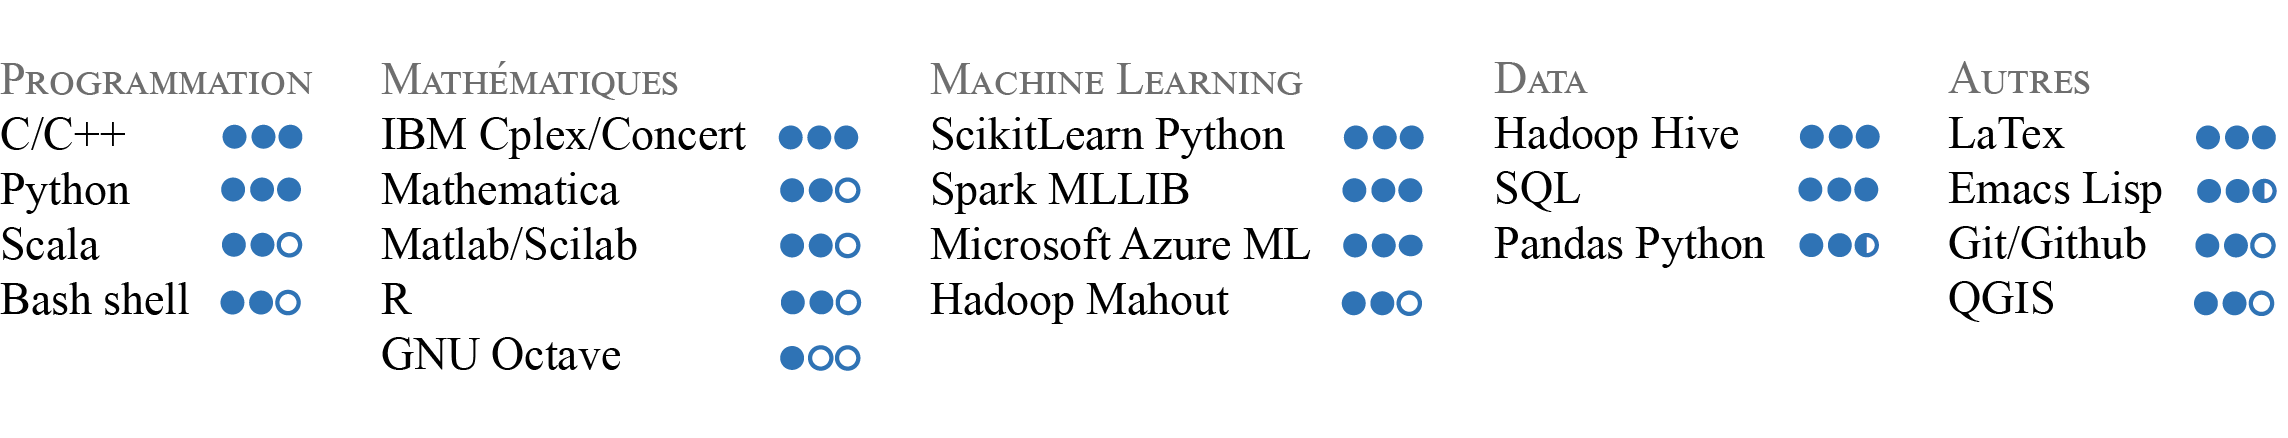
\includegraphics[trim= {0 2mm 0 5mm},clip,width=185mm]{Comp3107.png} \\
\end{minipage}

%\cvitem{}{\includegraphics[scale=0.81]{test.png}}
% \cvitem{\textcolor{color2bis}{OS}}{GNU/Linux, Mac OSX, Windows}

\cvitem{\textcolor{color2bis}{Langue}}{Anglais: capacité professionnelle complète}
%\cventry{year--year\\\includegraphics[width=\hintscolumnwidth]{test.png}}{Degree}{Institution}{City}{\textit{Grade}}{Description}

%\cvitem{\textcolor{color2bis}{Environements}}{\includegraphics[scale=1]{test.png}}
 %\cvitem{\textcolor{color2bis}{Environements}}{\includegraphics[scale=0.8]{test.png}}
%\cvitem{\textcolor{color2bis}{Programmation}}{C/C++, Python, Spark MLLIB,Microsoft Azure ML, Hadoop (Mahout, Hive), Scala, R, SQL, LaTeX, IBM
 % Cplex/Concert, Wolfram Mathematica, Matlab, Scilab, GNU Octave, Bash-shell,
  %QGIS, Git/Github, Emacs, \showthe\font}
  


\section{Formations}
\cventry{\textcolor{color2bis}{2014 -- 2016\\Septembre}}{Master Ingénierie Mathématiques (MIMSE)}{Université de Bordeaux}{}{}{
Spécialité Recherche Opérationnelle et Aide à la Décision: 
Optimisation mathématique, machine learning, théorie des graphes, C++ et Python approfondis, statistiques, analyse de données, base de données.\\
}
\cventry{\textcolor{color2bis}{2016\\Février-Avril}}{Certification Machine Learning}{Coursera}{}{}{MOOC Andrew Ng (note maximale 100\%)\newline{}}
\cventry{\textcolor{color2bis}{2011 -- 2012}}{Licence MASS}{Université de Toulon - Var}{}{}{Mathématiques Appliquées aux Sciences Économiques et Sociales incluant: statistiques, probabilités, économétrie, économie (micro/macro), sociologie, théorie de la décision. \newline{}}
\cventry{\textcolor{color2bis}{2008 -- 2011}}{Licence Mathématiques}{Université de Toulon - Var}{}{}{Mathématiques Pures incluant: algèbre (linéaire, théorie des groupes, anneaux, corps), analyse (réel, complexe, théorie de la mesure, calcul différentiel), géométrie (topologie), programmation. \newline{}}
% \cventry{\textcolor{color2bis}{2005 -- 2006}}{Baccalauréat}{Lycée Dumont d'Urville - Var}{}{}{Série Scientifique, spécialité Mathématiques. %\newline{}
}

\section{Centres d’intérêt}
\cvitem{\textcolor{color2bis}{Sciences}}{Participation au concours machine
  learning Cdiscount
  2015 'Catégorisation de produits pour le e-commerce'
  sur DataScience.net (place : 24 sur 830)}
\cvitem{\textcolor{color2bis}{Intérêts}}{Voyages et découverte des cultures et patrimoines, aïkido.}

\end{document}
%  LocalWords:  Ciblage
